\documentclass{article}
\usepackage[utf8]{inputenc}
\usepackage[margin=0.5in]{geometry}
\usepackage{graphicx} %package to manage images
\graphicspath{ {images/} }

\title{CS51 - Final Project Writeup}
\author{Matt Jiang}
\date{May 2, 2018}

\begin{document}

\maketitle

\section{Lexical Scope Extension}
For my final project extension, I implemented ``eval\_l", an evaluator that uses environment semantics like ``eval\_d" but provides closures for functions so that they use the environment they were created in (AKA the lexical environment). This is different from ``eval\_d", in which the functions use the environment at the time of application (AKA the dynamic environment). \\

Ocaml is lexically scoped, so ``eval\_l" handles expressions similarly to the native Ocaml interpreter. 

\subsection{``eval\_d" vs ``eval\_l}

The two are different in how they handle the Fun and App match cases. When ``eval\_l" evaluates a Fun case, instead of just returning the same Val (Fun expression), it returns a closure of the Fun expression and the env at the time. App in ``eval\_l" evaluates the function definition in the closure environment, as opposed to the current environment in ``eval\_d". Left is d, right is l.

\begin{center}
   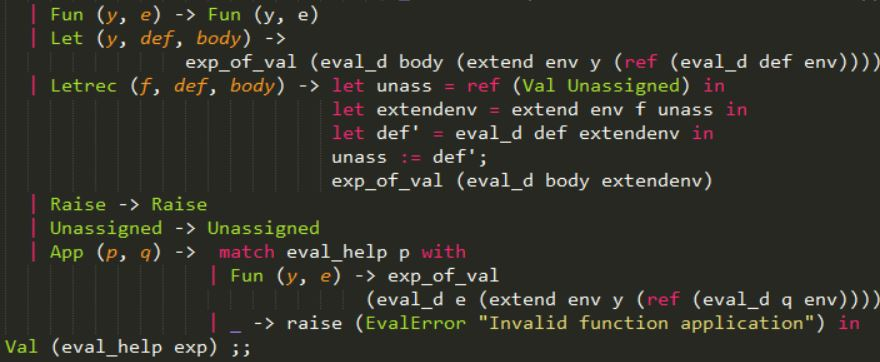
\includegraphics[scale=0.3]{Capture}    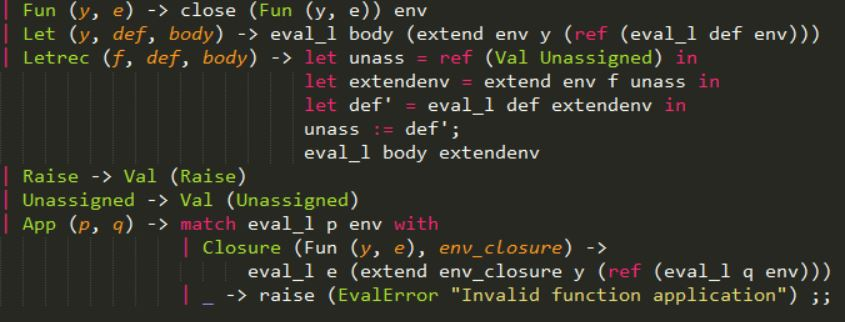
\includegraphics[scale=0.335]{1}
\end{center}

I also had to change how extend works. Initially, it reassigned the reference of the id it was extending; however, this would also change instances inside closures, which was undesirable. I fixed it by making it find elements of the environment whose first element matched the id (so only within the general environment), then deleting those and replacing them with a new element containing the id and the new value ref.

\subsection{an example}

\begin{center}
let x = 1 in
let f = fun y -$>$ x + y in
let x = 2 in
f 3 ;;\end{center}
\\


d will only evaluate f when it is being applied in the current environment. So when f is applied to 3 in the environment where x = 2, f evaluates to fun y -$>$ 2 + y, and f 3 to 5. 

l saves f in a closure the first time it is encountered, along with the environment at that time (i.e. x = 1). When it hits the next line ``x = 2", this extends the general environment but does not affect the closure environment. So when f 3 is evaluated, f is evaluated in its closure environment to fun y -$>$ 1 + y, and f 3 to 4.


\end{document}
